\documentclass[a4paper, 10pt, conference]{ieeeconf}

\IEEEoverridecommandlockouts
\overrideIEEEmargins

\usepackage{graphics} % for pdf, bitmapped graphics files
\usepackage{epsfig} % for postscript graphics files
\usepackage{mathptmx} % assumes new font selection scheme installed
\usepackage{times} % assumes new font selection scheme installed
\usepackage{amsmath} % assumes amsmath package installed
\usepackage{amssymb}  % assumes amsmath package installed
\usepackage{hyperref}
\usepackage{listings}
\usepackage{subfigure}

\usepackage[T1]{fontenc}
\usepackage[utf8]{inputenc}
\usepackage[brazil]{babel}
\usepackage{etoolbox}
\patchcmd{\abstract}{Abstract}{Resumo}{}{}
\patchcmd{\thebibliography}{References}{Referências}{}{}

\title{\LARGE \bf Uma linguagem de programação para processamento de imagens}

\author{Henrique Miyamoto e Thiago Benites}

\begin{document}
\maketitle
\thispagestyle{empty}
\pagestyle{empty}

%\begin{abstract}

%Escreva aqui o resumo (abstract).

%\end{abstract}

\section{Contextualização}

%Um breve texto introdutório explicando do que se trata o documento, em uma linguagem que poderia ser entendida por qualquer pessoa que entenda programação (ou seja: referências diretas à disciplina não são desejáveis).

Apresentamos uma linguagem de programação voltada para o processamento de imagens digitais. Ela foi implementada com um analisador léxico e utilizando de gramática livre de contexto. Como uma linguagem de programação de propósito específico, seu objetivo é ser intuitiva para o usuário \cite{dsl}. As funcionalidades que nossa linguagem é capaz de executar, assim como as respectivas sintaxes são apresentadas na Tabela \ref{tabela1}.

\begin{table}[h]
	\centering
	\caption{Funcionalidades e sintaxe da linguagem de programação}
	\label{tabela1}
	\begin{tabular}{|c|c|}
		\hline
		\textbf{Funcionalidade}        & \textbf{Sintaxe}                                                                                                                \\ \hline
		Salvar uma imagem     & {destino.jpg = origem.jpg}                                                                                    \\ \hline
		Alterar brilho        & \begin{tabular}[c]{@{}c@{}}{destino.jpg = origem.jpg * float}\\ {destino.jpg = origem.jpg / float}\end{tabular} \\ \hline
		Detectar valor máximo & {[origem.jpg]}                                                                                            \\ \hline
	\end{tabular}
\end{table}

Nos processos de salvar uma imagem e de alterar seu brilho, é feita uma cópia do arquivo original. Calculamos o valor de cada pixel como a intensidade na conversão do espaço RGB para o HSI $I=\frac{1}{3}(R+G+B)$ \cite{rgb} na detecção do valor máximo da imagem.

\section{Demonstração}

%Entradas e saídas que demonstram as funcionalidades implementadas.

Para demonstração das funcionalidades, tomemos por base a imagem em sua forma original apresentada na Figura \ref{fig1}. Quando aplicado brilho de fator multiplicativo 2, tem-se o resultado apresentado na Figura \ref{fig2}. Já ao dividir pelo mesmo fator, obtém-se o resultado da Figura \ref{fig3}.

\begin{figure}[h]
	\centering
	\subfigure[]{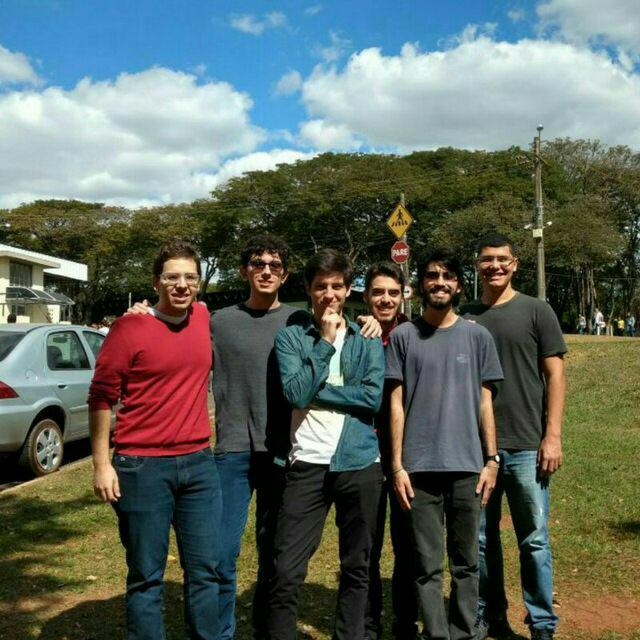
\includegraphics[width=2.7cm]{Figuras/figura1}\label{fig1}}
	\hspace{0.05cm}
	\subfigure[]{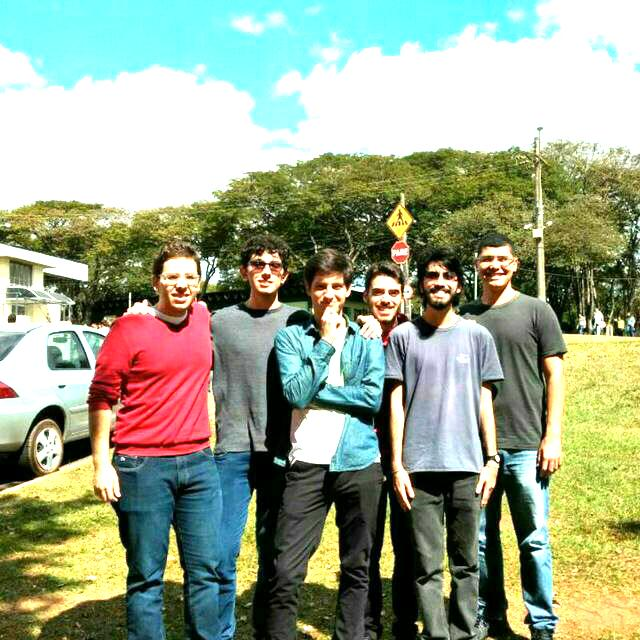
\includegraphics[width=2.7cm]{Figuras/figura2}\label{fig2}}
	\hspace{0.05cm}
	\subfigure[]{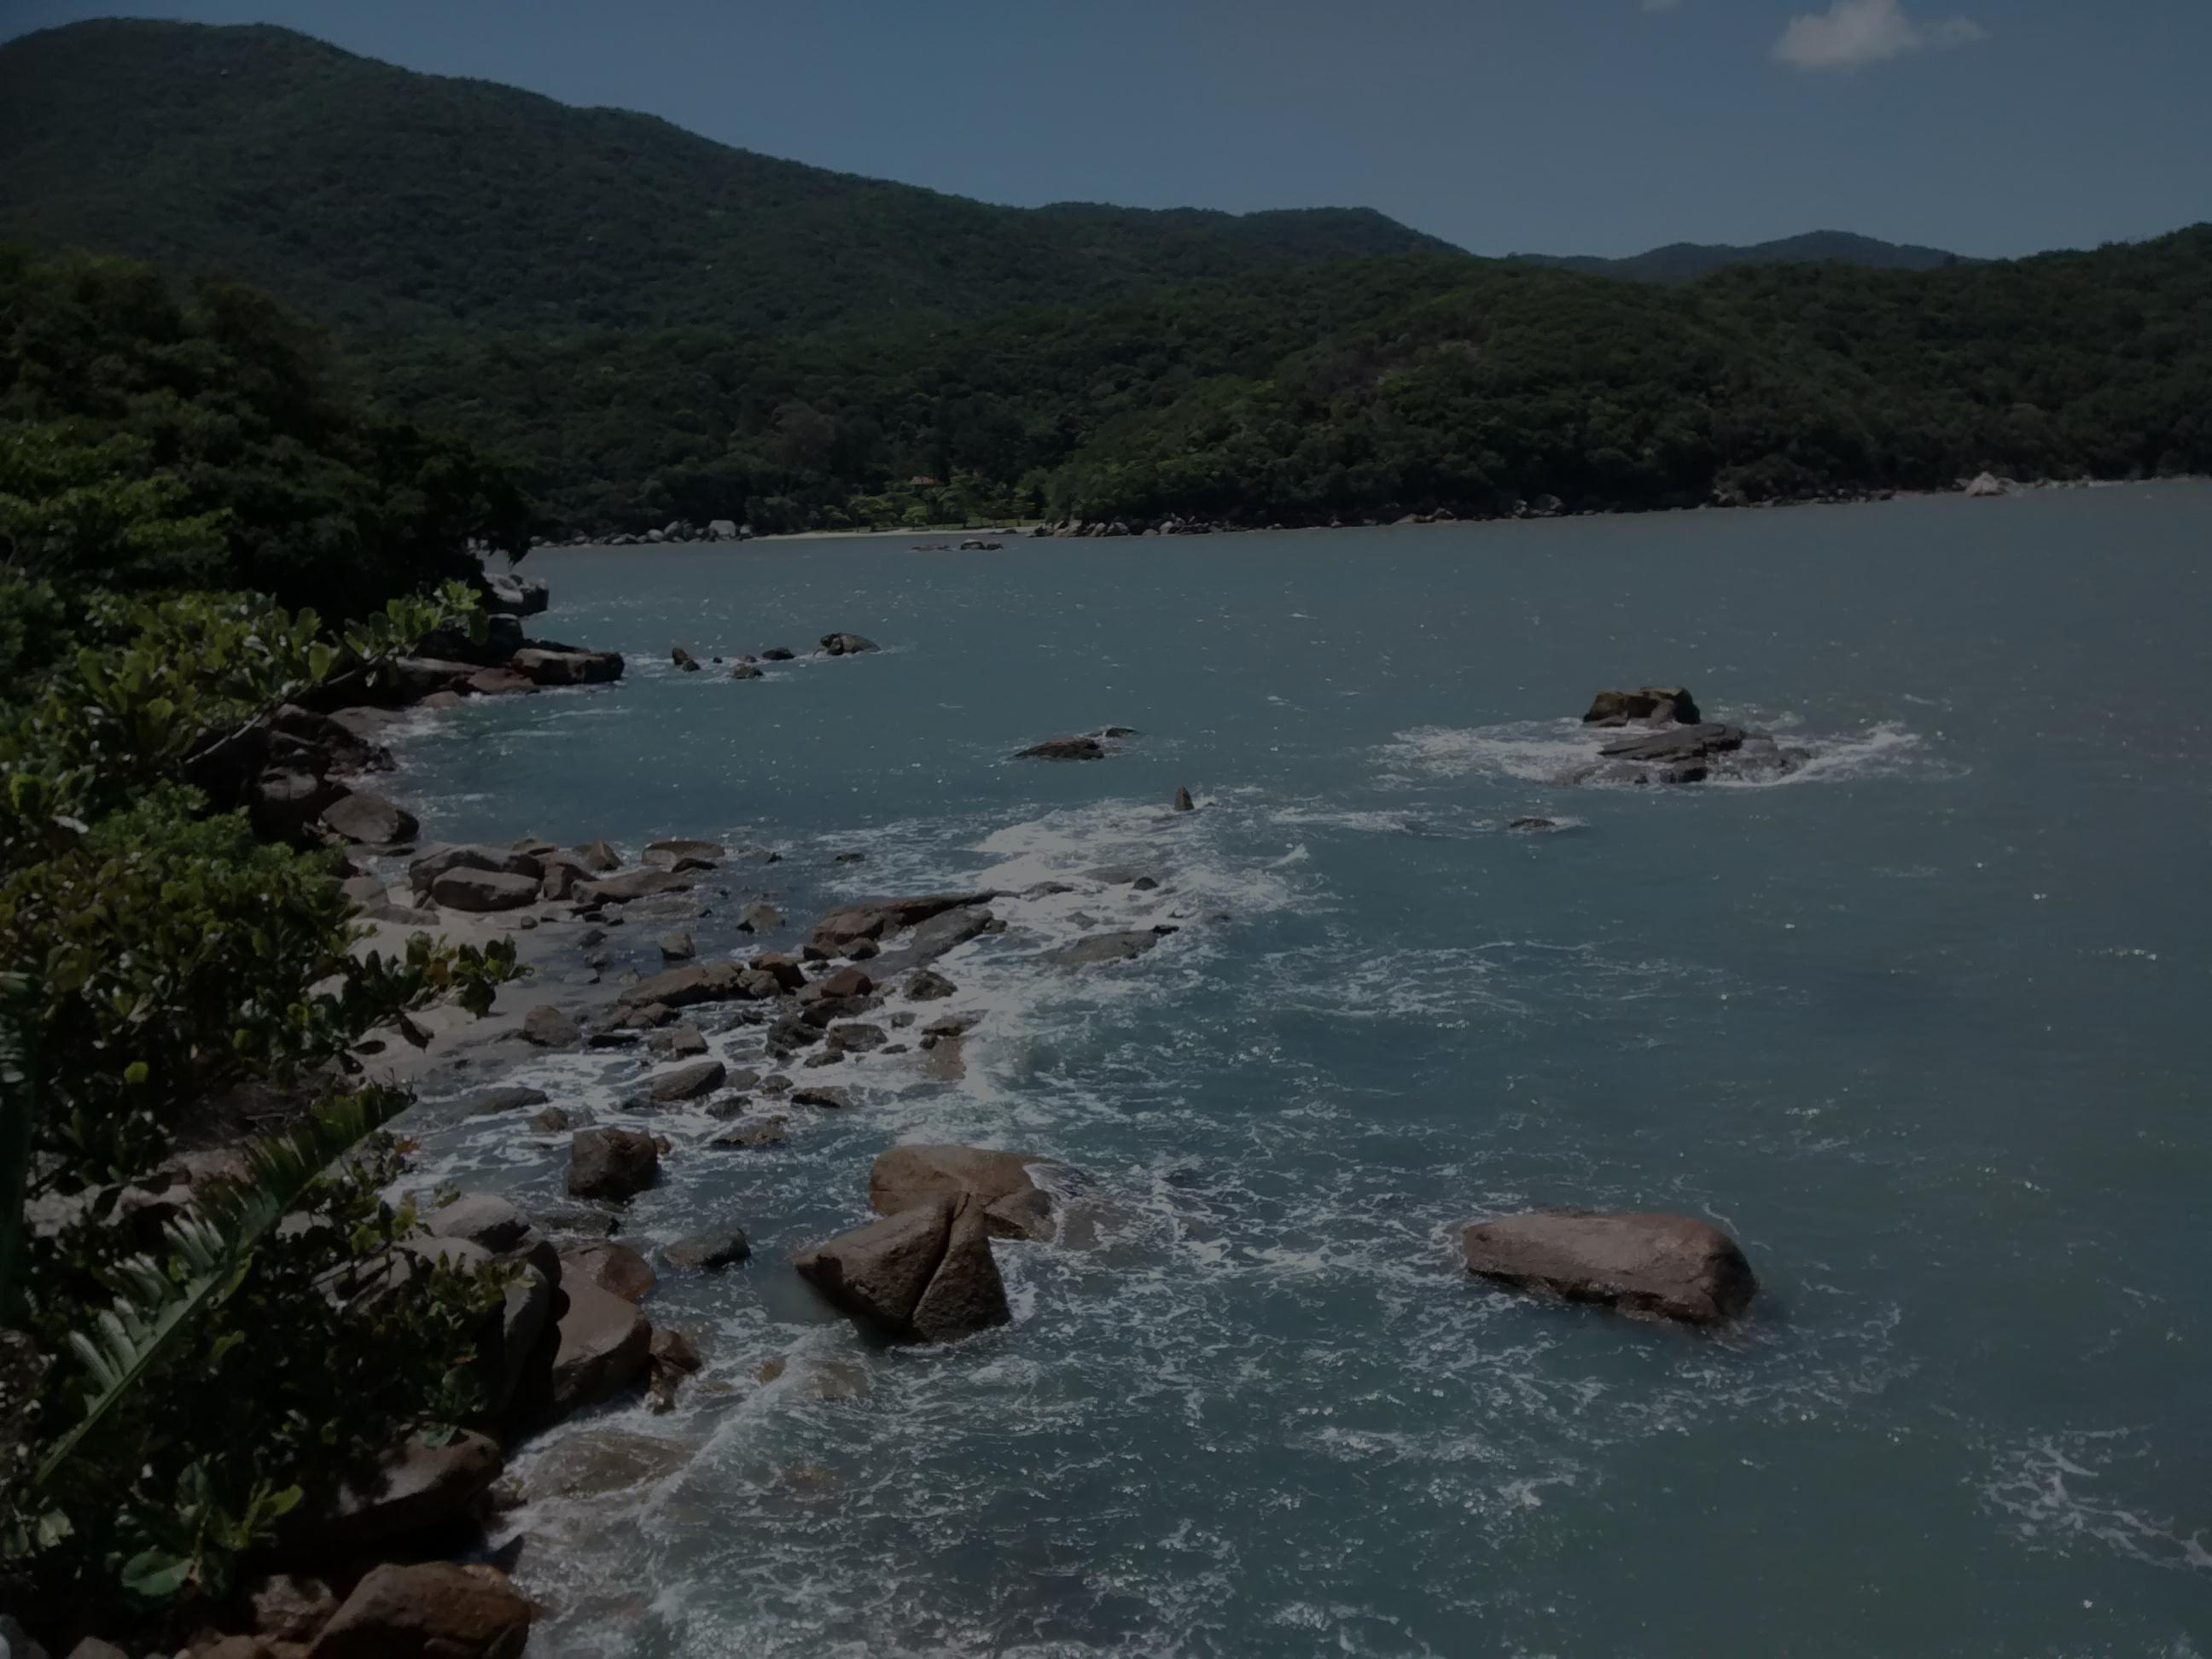
\includegraphics[width=2.7cm]{Figuras/figura3}\label{fig3}}
	\caption{Imagens: (a) original, (b) com brilho dobrado e (c) reduzido à metade.}
	\label{comp}
\end{figure}

Para as três figuras é possível aplicar a função que detecta o máximo valor de brilho, de acordo com a seguinte implementação e resultados:
\newline
\newline
\newline
\begin{lstlisting}[language=C, basicstyle=\footnotesize, frame=single]
./main
[figura1.jpg]
Intensidade maxima: 254.00
[figura2.jpg]
Intensidade maxima: 255.00
[figura3.jpg]
Intensidade maxima: 133.00
\end{lstlisting}

\section{Análise}

%Comparando a idéia de usar os comandos específicos da linguagem para aplicar brilho com uma aplicação equivalente, usando alguma biblioteca de linguagem de propósito geral (por exemplo, `OpenCV`). A análise deve se basear em dados reais, e mostrar todos os dados sobre os quais ela se baseia (exemplos de código, citações bibliográficas ou outros dados que o grupo considere relevantes).

Comparamos a ideia de usar um comando específico para alterar o brilho com aplicações equivalentes de propósito geral, como OpenCV. Em sua versão para C++, a aplicação de brilho a uma imagem pode ser feita através do comando convertTo(), com a seguinte sintaxe \cite{opencv2}:
\begin{lstlisting}[language=C, basicstyle=\footnotesize]
void Mat::convertTo(OutputArray m, int rtype, 
double alpha=1, double beta=0 ) const
\end{lstlisting}
em que alpha e beta são fatores de escala que realizam a operação linear $g(x)=\alpha f(x) + \beta$, sobre a imagem $f(x)$, resultando na imagem $g(x)$ \cite{opencv}.

O comando utilizado na nossa linguagem para tal função é mais simples, no sentido de que tem menos argumentos e lida com menos conceitos de programação que os outros dois, exigindo menos conhecimento do usuário. Por exemplo, no comando do OpenCV, é necessário entender que aplica-se uma transformação linear à imagem, com parâmetros que definem contraste e brilho, além de lidar com a imagem na forma matricial. Na nossa sintaxe, é necessário utilizar apenas os nomes dos arquivos e a intensidade de brilho que se deseja aplicar, ficando oculto para o usuário final o formato como a imagem é tratada e procedimentos realizados.

Se por um lado comandos como o do OpenCV possam gerar maior flexibilidade para usuários avançados, sintaxes mais diretas oferecem ganho em expressividade e facilidade no uso, principalmente quando comparadas à linguagens de uso geral \cite{dsl}.

\begin{thebibliography}{99}

\bibitem{dsl} When and How to Develop Domain-Specific Languages. MERNIK, Marjan; HEERIN, Jan; SLOANE, M Anthony. Disponível em: \url{https://pdfs.semanticscholar.org/bd06/01088d5f217dc136a898f577763df92891cb.pdf}. Acesso em: 17 set. 2017.


\bibitem{rgb} Wikipedia. RGB color model. Disponível em: \url{https://en.wikipedia.org/wiki/RGB_color_model}. Acesso em: 10 set. 2017.

\bibitem{opencv2} OpenCV. Basic Structures. Disponível em: \url{http://docs.opencv.org/2.4/modules/core/doc/basic_structures.html}. Acesso em: 11 set. 2017.

\bibitem{opencv} OpenCV. Changing the contrast and brightness of an image!. Disponível em: \url{http://docs.opencv.org/2.4/doc/tutorials/core/basic_linear_transform/basic_linear_transform.html}. Acesso em: 11 set. 2017.

\end{thebibliography}

\end{document}